\chapter{Erweiterte Funktionen}\label{ch:erweitert}

\section{Adaptive räumliche Auflösung (ASR)}\label{sec:asr}
\index{ASR}\index{Koordinatentransformation}%
Bei Metallstrukturen in TM konzentriert sich das Feld an den Kanten; dort braucht die Fourierreihe die meisten
Ordnungen. Die adaptive räumliche Auflösung nach Granet verzerrt die Koordinate $x$ (und $z$) so, dass die
Fourierbasis an den Materialsprüngen feiner auflöst. Die Zahl der Ordnungen bleibt gleich, die Konvergenz wird
deutlich schneller.
\begin{lstlisting}[language=json]
"coordinate_transform": {
  "x": { "type": "asr", "eta": 0.9, "breakpoints_um": "auto" },
  "z": { "type": "asr", "eta": 0.5, "breakpoints_um": [0.1, 0.4] }     // nur 2D
}
\end{lstlisting}
\begin{center}
\small
\begin{tabularx}{\linewidth}{llY}
\toprule
Schlüssel & Standard & Bedeutung \\
\midrule
\key{type} & -- & \val{"asr"} \\
\key{eta} & 0 & Verdichtung $0\le\eta<1$; das Raster wird an den Stellen um den Faktor $1-\eta$ feiner. $\eta=0$ ist
keine Transformation (bitgleich zur Rechnung ohne Block) \\
\key{breakpoints\_um} & \val{"auto"} & Stellen der Verdichtung: \val{"auto"} nimmt alle Materialsprünge der
Lamellenschichten und die Eckkoordinaten der Polygone; oder eine Liste \\
\bottomrule
\end{tabularx}
\end{center}
\begin{itemize}
  \item Empfehlung für Metall-Lamellen in TM: $\eta=0{,}8$ bis $0{,}95$. Das Beispiel in
        Abschnitt~\ref{sec:konvergenz} zeigt: Mit $\eta=0{,}95$ ist $e_{-1}$ eines Goldgitters ab $N=20$ auf vier Stellen
        genau, ohne ASR auch bei $N=80$ nicht.
  \item Bei Profilschichten gibt es keine Sprünge, die \val{"auto"} finden könnte; geben Sie dann eine Liste an,
        sonst meldet \FG{} \texttt{no material jumps found along the axis, give breakpoints\_um}.
  \item Mit einer einzigen Stelle ist die Abbildung analytisch (schnellste Konvergenz). Bei mehreren ungleich langen
        Intervallen konvergiert die Rechnung algebraisch ($\sim N^{-5}$).
  \item Mit ASR wird \key{split\_polarizations} nicht genutzt; ASR und PML schließen sich aus.
  \item Im Nahfeld bleibt die Ausgabe auf dem physikalischen Raster; nur die Fourierkoeffizienten
        (\texttt{fieldCoefficients}) beziehen sich auf die transformierten Koordinaten.
\end{itemize}

%-------------------------------------------------------------------------------------------
\section{Isolierte Strukturen mit PML}\label{sec:pml}
\index{PML}\index{isolierte Struktur}\index{Streufeld}%
Ein einzelner Steg, ein Graben, ein Kontaktloch oder ein Wellenleiterende ist nicht periodisch. \FG{} rechnet ihn in
einer Rechenzelle mit \textbf{absorbierenden Randzonen} (perfectly matched layers, PML): Am Zellrand wird die
Koordinate komplex gestreckt, sodass auslaufende Wellen dort ohne Reflexion abklingen. Die Nachbarzellen sehen sich
dann nicht mehr.
\begin{center}
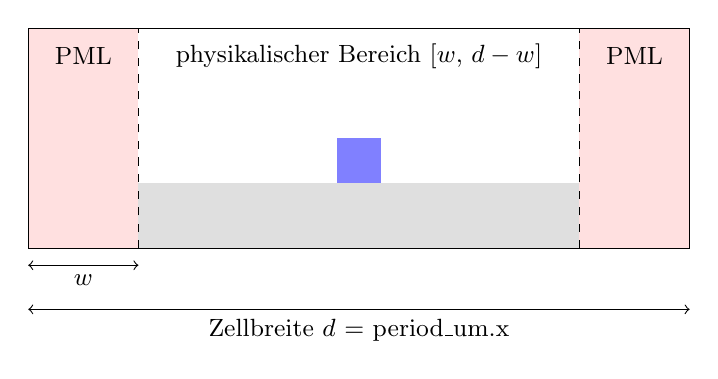
\begin{tikzpicture}[scale=1.4]
  \fill[gray!25] (0,-0.6) rectangle (6,0);
  \fill[red!12] (0,-0.6) rectangle (1,1.4);
  \fill[red!12] (5,-0.6) rectangle (6,1.4);
  \fill[blue!50] (2.8,0) rectangle (3.2,0.4);
  \draw (0,-0.6) rectangle (6,1.4);
  \draw[dashed] (1,-0.6) -- (1,1.4); \draw[dashed] (5,-0.6) -- (5,1.4);
  \node at (0.5,1.15) {\small PML}; \node at (5.5,1.15) {\small PML};
  \node at (3,1.15) {\small physikalischer Bereich $[w,\,d-w]$};
  \draw[<->] (0,-0.75) -- (1,-0.75) node[midway,below] {\small $w$};
  \draw[<->] (0,-1.15) -- (6,-1.15) node[midway,below] {\small Zellbreite $d$ = \key{period\_um.x}};
\end{tikzpicture}
\end{center}
\begin{lstlisting}[language=json]
"aperiodic": {
  "pml": { "x": { "width_um": 0.8, "beta": 1.0 },
           "z": { "width_um": 0.8 } },       // z nur in 2D
  "formulation": "auto",                     // oder "scattered"
  "excitation": "plane_wave"                 // oder {"mode": 0} bzw. {"n_eff": 1.9}
}
\end{lstlisting}
\begin{center}
\small
\begin{tabularx}{\linewidth}{llY}
\toprule
Schlüssel & Standard & Bedeutung \\
\midrule
\key{pml.x.width\_um} & -- & Breite $w$ der Randzone an beiden Zellenden \\
\key{pml.x.beta} & 1,0 & Stärke der Absorption \\
\key{formulation} & \val{auto} & \val{auto}: Totalfeld bei Normaleinfall, Streufeld bei schrägem Einfall;
\val{scattered}: immer Streufeld \\
\key{excitation} & \val{plane\_wave} & oder geführte Mode eines strukturierten Superstrats (siehe unten) \\
\bottomrule
\end{tabularx}
\end{center}
\paragraph{Regeln.}
\begin{itemize}
  \item Strukturen dürfen nicht in die PML-Zonen reichen (geprüft, auch für CAD-Schnitte). Durchgehende Filme
        (homogene Schichten) dürfen durchlaufen.
  \item Die Zellbreite muss deutlich größer sein als die Struktur. Bei gleicher Auflösung wächst die nötige
        Ordnungszahl $N$ proportional zur Zellbreite; prüfen Sie Konvergenz in $N$ \emph{und} in der Zellbreite.
  \item PML und ASR schließen sich aus.
\end{itemize}

\paragraph{Ausgabe.} Statt Beugungseffizienzen gibt es Streugrößen, bezogen auf die Intensität der einfallenden
Welle (1D: Streubreite in \textmu m, 2D: Streuquerschnitt in \textmu m$^2$):
\begin{lstlisting}
lambda = 0.6328 um, phi = 0 deg, psi = 0 deg, delta = 0 deg
  side   n    m   efficiency
  scattered up = 0.3289787262   down = 0.3704020556   absorbed = 0.02285324735   (um, 2D: um^2)
\end{lstlisting}
Das ist ein 0,3\um{} breiter Siliziumsteg (0,2\um{} hoch) auf Glas in einer 4\um{} breiten Zelle mit 0,8\um{} PML
($N=60$, Rechenzeit etwa 8\,s). In der CSV-Datei heißen die Zeilen \texttt{S\_up}, \texttt{S\_down},
\texttt{S\_abs}; in Python \texttt{res.scattering} mit den Schlüsseln \texttt{up}, \texttt{down}, \texttt{lateral},
\texttt{absorbed}.
\begin{itemize}
  \item \texttt{up}/\texttt{down}: Leistung des Streufeldes durch die Ebenen oberhalb und unterhalb der Struktur über
        den physikalischen Bereich.
  \item \texttt{lateral}: durch die Seiten der Box; \texttt{absorbed}: in der Box absorbiert.
  \item Nur die Summe \texttt{up + down + lateral} ist unabhängig von der Zellbreite. Die Aufteilung oben/unten
        konvergiert bei schrägem Einfall langsam ($\sim1/L$).
\end{itemize}

\paragraph{Totalfeld und Streufeld.} Bei senkrechtem Einfall rechnet \FG{} das Totalfeld und zieht den
Hintergrund ab (jede strukturierte Schicht ersetzt durch ihr Material am Zellrand). Bei schrägem Einfall wäre die
einfallende Welle nicht periodisch; dann verwendet \FG{} automatisch die \textbf{Streufeldformulierung}: Der
Hintergrund wird analytisch gelöst, die Struktur wirkt als Quelle $\sigma=(M-M_{\text{bg}})F_{\text{bg}}$. Mit
\val{"nearfield": \{"field": "scattered"\}} geben Sie im Nahfeld nur das Streufeld aus.

\subsection{Anregung durch eine geführte Mode}
Ein strukturierter Halbraum (z.\,B.\ ein Wellenleiter, der in $y$-Richtung läuft) kann eine Mode einspeisen; berechnet
werden die Leistungen der reflektierten und transmittierten Moden. Typische Anwendung: Wellenleiterenden,
Taper, Gitterkoppler.
\begin{lstlisting}[language=json]
"aperiodic": { "pml": { "x": { "width_um": 0.5 } }, "excitation": { "mode": 0 } },
"superstrate_structure": { "type": "lamellar1d",
                           "breakpoints_um": [0, 1.3, 1.7, 3.0],
                           "materials": ["air", "core", "air"] },
"substrate_structure": { ... }
\end{lstlisting}
\begin{itemize}
  \item \key{superstrate\_structure}, \key{substrate\_structure}: $y$-invariante Querschnitte (\val{lamellar1d},
        \val{polygon2d}, \val{contour2d}) der Halbräume; die Dicke entfällt. \key{superstrate}/\key{substrate} nennen dann
        den Mantel.
  \item \key{excitation}: \val{\{"mode": k\}} wählt die $k$-te geführte Mode nach absteigendem effektivem Index,
        \val{\{"n\_eff": x\}} die Mode mit dem nächstgelegenen Index.
  \item Ausgabe: \texttt{MR}/\texttt{MT} je Mode (Modennummer und Leistung), \texttt{Mrad} (abgestrahlt); Python
        \texttt{res.modal}.
\end{itemize}

\subsection{Streufeldformulierung für periodische Gitter}
\val{"scattered\_field": true} erzwingt die Streufeldformulierung auch bei periodischen Gittern. Die Effizienzen sind
dann die von Hintergrund plus Streufeld; das Ergebnis ist dasselbe wie ohne. Gedacht ist die Option für Tests
(Referenzfall V20d).

%-------------------------------------------------------------------------------------------
\section{Rotationssymmetrische Strukturen (in Arbeit)}\label{sec:zylinder}
\index{Zylinderkoordinaten}\index{Gauß-Strahl}%
Säulen, Scheiben, Löcher, Ringe und Zonenplatten auf einem Schichtstapel sind rotationssymmetrisch um eine Achse
senkrecht zum Stapel. In Zylinderkoordinaten entkoppeln die azimutalen Harmonischen $e^{im\varphi}$; je Harmonischer
bleibt ein Problem in $(r,y)$. Das ist viel günstiger, als die isolierte Struktur kartesisch mit PML zu rechnen.

\begin{achtung}[Stand]
Meilenstein M20 ist teilweise umgesetzt: Schichttypen \val{homogeneous}, \val{rings} und \val{rings\_profile},
isotrope Materialien, Gauß-Strahlen auf der Achse und ebene Wellen (Streufeld), Leistungen, Streu-, Absorptions- und
Extinktionsquerschnitt, Nahfeld, Winkelspektrum und Fernfeld, CAD-Rotationskörper
(Abschnitt~\ref{sec:cad-axisym-hb}).
\end{achtung}

\begin{lstlisting}[language=json]
{
  "cylindrical": {
    "symmetry": "axial",
    "harmonics": "auto",                                   // oder Liste, z. B. [-1, 1]
    "spectrum": { "kappa_max": 4, "dk_factor": 1.0, "deform": "auto" },
    "factorization": "li_r"                                // oder "laurent"
  },
  "solver": "rcwa",
  "materials": { "air": {"n": 1.0}, "glass": {"n": 1.5}, "sin": {"n": 1.45} },
  "superstrate": "air", "substrate": "glass",
  "incidence": { "type": "gaussian_beam", "lambda_um": [0.9, 1.0, 1.1],
                 "waist_um": 0.5, "focus_y_um": 0.8, "polarization": "x" },
  "layers": [ { "type": "rings", "thickness_um": 0.3, "radii_um": [0.4],
                "materials": ["sin", "air"] } ],
  "output": { "dir": "out_cyl_pillar_beam" }
}
\end{lstlisting}
\begin{center}
\small
\begin{tabularx}{\linewidth}{llY}
\toprule
Schlüssel & Standard & Bedeutung \\
\midrule
\key{symmetry} & \val{axial} & Rotationssymmetrie ($P$-zählige Symmetrie folgt mit M21) \\
\key{harmonics} & \val{auto} & azimutale Ordnungen $m$; \val{auto}: $m=\pm1$ bei Strahl/Normaleinfall, sonst
$|m|\le m_{\text{cut}}$ \\
\key{spectrum.kappa\_max} & & obere Grenze des Hankel-Spektrums (in Einheiten von $k_0$) -- der Genauigkeitsparameter \\
\key{spectrum.dk\_factor} & 1,0 & Feinheit der Stützstellen; um Plasmonen eines Metallfilms zwischen verschiedenen Halbräumen wird automatisch verfeinert \\
\key{spectrum.nodes\_per\_panel} & 8 & Gauß-Knoten je Teilintervall \\
\key{spectrum.deform} & \val{auto} & komplexer Integrationsweg um Verzweigungspunkte: \val{auto}, \val{false} oder
\val{\{"delta": 0.05\}} \\
\key{factorization} & \val{li\_r} & \val{li\_r} (Li-Regel in $r$) oder \val{laurent} \\
\key{optical\_theorem} & \val{false} & ebene Welle: optisches Theorem als Kontrolle (\texttt{C\_Sext\_ot}); kostet
etwa die doppelte Rechenzeit, bei verlustbehafteten Ringen ohnehin berechnet \\
\key{far\_field.n\_phi} & -- & Fernfeld auf so vielen Azimuten, dazu \texttt{angular\_spectrum.csv} und
\texttt{far\_field.csv} \\
\bottomrule
\end{tabularx}
\end{center}
\paragraph{Schichten mit veränderlichem Radius.} \val{rings\_profile} beschreibt Kegelstümpfe, Kugeln, Kugelkappen
und beliebige Rotationsprofile: Jeder Radius ist eine Zahl, \val{\{"cone": [r0, r1]\}} (unten, oben),
\val{\{"sphere": \{"center\_y\_um": c, "radius\_um": R\}\}} ($y$ ab der Schichtunterkante) oder eine Tabelle
\val{\{"table": \{"y\_um": [...], "r\_um": [...]\}\}}. Gerechnet wird eine Treppe aus \key{slices} Scheiben mit den
Radien in der Scheibenmitte; der Treppenfehler fällt etwa mit $1/K^2$, prüfen Sie die Konvergenz in \key{slices}.
\begin{lstlisting}[language=json]
{ "type": "rings_profile", "thickness_um": 0.6, "slices": 20,
  "radii": [ { "sphere": { "center_y_um": 0.3, "radius_um": 0.3 } } ],
  "materials": ["sin", "air"] }
\end{lstlisting}
\paragraph{Einfall.}
\begin{itemize}
  \item \val{gaussian\_beam}: \key{lambda\_um}, \key{waist\_um} (Strahltaille), \key{focus\_y\_um} (Lage des Fokus),
        \key{polarization}: \val{x}, \val{z}, \val{circular\_plus}, \val{circular\_minus}, \val{radial},
        \val{azimuthal}. Winkel sind nicht erlaubt (Strahl auf der Achse).
  \item \val{plane\_wave}: Winkel wie beim kartesischen Einfall, Polarisation über \key{delta\_deg}; Strahlparameter
        sind nicht erlaubt. Gerechnet wird in der Streufeldformulierung.
\end{itemize}
\paragraph{Ausgabe.} Mit dem Beispiel oben:
\begin{lstlisting}
lambda_um,...,side,n,m,efficiency,...
0.9,...,C_R,0,0,0.0474282286936,...
0.9,...,C_T,0,0,0.952447477038,...
0.9,...,C_A,0,0,0.000124294268031,...
0.9,...,C_Rm,-1,0,0.0237141143468,...
0.9,...,C_Tm,-1,0,0.476223738519,...
\end{lstlisting}
\texttt{C\_R}, \texttt{C\_T} sind die reflektierte und transmittierte Leistung relativ zum Strahl, \texttt{C\_A}
$=1-R-T$ (enthält auch den seitlichen Abfluss in geführte Moden). \texttt{C\_Rm}, \texttt{C\_Tm} zerlegen nach
Harmonischen. Bei der ebenen Welle stehen Streuquerschnitte in \textmu m$^2$ in \texttt{C\_Sup}, \texttt{C\_Sdown},
\texttt{C\_Ssca}, dazu der Absorptionsquerschnitt \texttt{C\_Sabs} ($\tfrac1{2I_{\text{inc}}}\int\operatorname{Im}\varepsilon
|\mathbf E|^2\,dV$ über die Ringe), \texttt{C\_Sext} $=$ \texttt{C\_Ssca} $+$ \texttt{C\_Sabs} und zur Kontrolle
\texttt{C\_Sext\_ot} (optisches Theorem; mit \key{optical\_theorem} oder verlustbehafteten Ringen, nicht bei
absorbierendem Hintergrund). Weicht \texttt{C\_Sext\_ot}
deutlich von \texttt{C\_Sext} ab, ist die Rechnung nicht konvergiert. Bei einem Strahl auf verlustbehafteten Ringen
steht in Python \texttt{res.cylindrical["absorbed\_rings"]} die in den Ringen absorbierte Leistung; die Differenz zu
\texttt{C\_A} ist der seitliche Abfluss. Mit \val{"scattered\_field": true} rechnet auch ein Strahl in der
Streufeldformulierung; das Ergebnis ist dasselbe wie beim Totalfeld (eine Kontrolle der Quellen, keine andere Physik).
Python: \texttt{res.cylindrical}. Rechenzeit des Beispiels: etwa 14\,s für
drei Wellenlängen auf zwei Kernen. Konvergenz prüfen Sie über \key{kappa\_max} und \key{dk\_factor}.

\begin{achtung}[Kleine Metallteilchen]
$k_{\max}=\kappa_{\max}\max\operatorname{Re}n$ richtet sich nach dem größten Realteil der Brechzahl. Bei Metallen
($\operatorname{Re}n<1$) und Teilchen, die klein gegen die Wellenlänge sind, braucht es deshalb ein großes
\key{kappa\_max}: $k_{\max}R$ sollte mindestens 15 sein ($R$: Teilchenradius in Einheiten von $1/k_0$). Eine Goldkugel
als Treppe aus Scheiben trifft die Extinktion schnell, die Aufteilung in Streuung und Absorption konvergiert langsam
(Abschnitt~\ref{sec:zylinder_nf}).
\end{achtung}

\paragraph{Winkelspektrum und Fernfeld.}
Jede Rechnung liefert in Python \texttt{res.cylindrical["angular\_spectrum"]}: je Harmonischer $m$ und Seite
(\val{up} ins Superstrat, \val{down} ins Substrat, wenn es verlustfrei ist) die abgestrahlte Leistung je Winkel
$dP/d\theta$ an den Stützstellen des Spektrums ($\theta=\arcsin(k/n)$), getrennt nach s (TE) und p (TM), und das
Quadraturgewicht \texttt{weight}; $\sum\texttt{weight}\cdot(s+p)$ ist die Leistung der Harmonischen
(\texttt{C\_Rm}, \texttt{C\_Tm} bzw.\ \texttt{C\_Supm}, \texttt{C\_Sdownm}). Mit
\val{"far\_field": \{"n\_phi": 72\}} im Block \key{cylindrical} kommt das Fernfeld $dP/d\Omega$ auf (Winkel $\theta$)
$\times$ (72 Azimute) hinzu; \texttt{fgsolve} schreibt dann \texttt{angular\_spectrum.csv} und \texttt{far\_field.csv}.
Beim Strahl ist alles auf die einfallende Leistung bezogen, bei der ebenen Welle ist es der differentielle
Streuquerschnitt in \textmu m$^2$ je Steradiant. Eine kleine Kugel trifft die Mie-Lösung auf $0{,}5\,\%$ des
Maximums ($\kappa_{\max}=8$).

\paragraph{Nahfeld.}\label{sec:zylinder_nf}
Der Block \key{nearfield} (Abschnitt~\ref{ch:nahfeld}) gilt auch hier. Der horizontale Schnitt ist eine Karte in $x$
und $z$, der vertikale Schnitt die Ebene $z=$\,\key{vertical\_z\_um} ($z=0$: Schnitt durch die Achse). $x$ und $z$ laufen
symmetrisch über $[-$\key{extent\_um}$,\,$\key{extent\_um}$]$ mit \key{nx} bzw.\ \key{nz} Punkten einschließlich der
Ränder; Standard ist das 1,5-Fache des äußeren Radius $R_s$, \key{periods} entfällt. Strahlen liefern das Totalfeld,
ebene Wellen Total- oder Streufeld (\key{field}). Mit \val{"reconstruction": "fff"} und Li in $r$ ist die
Normalkomponente $D_r$ an den Ringwänden stetig, $E_r$ springt; \val{direct} glättet den Sprung (Gibbs). Jenseits
von etwa $2R_s$ wird die Synthese ungenauer (die Stützstellendichte ist auf $R_s$ abgestimmt).
\begin{lstlisting}[language=json]
"nearfield": { "enabled": true, "horizontal_y_um": 0.15, "vertical_z_um": 0.0,
               "y_range_um": [-0.3, 1.0], "nx": 201, "ny": 131, "nz": 201, "extent_um": 1.0 }
\end{lstlisting}
